\chapter{Additions to the application}\label{chpt:applicationAdditions}
\glsresetall

\section{Architecture of Yolov5}\label{sec:aa:archyolov5}

\begin{figure}[H]
	\centering
	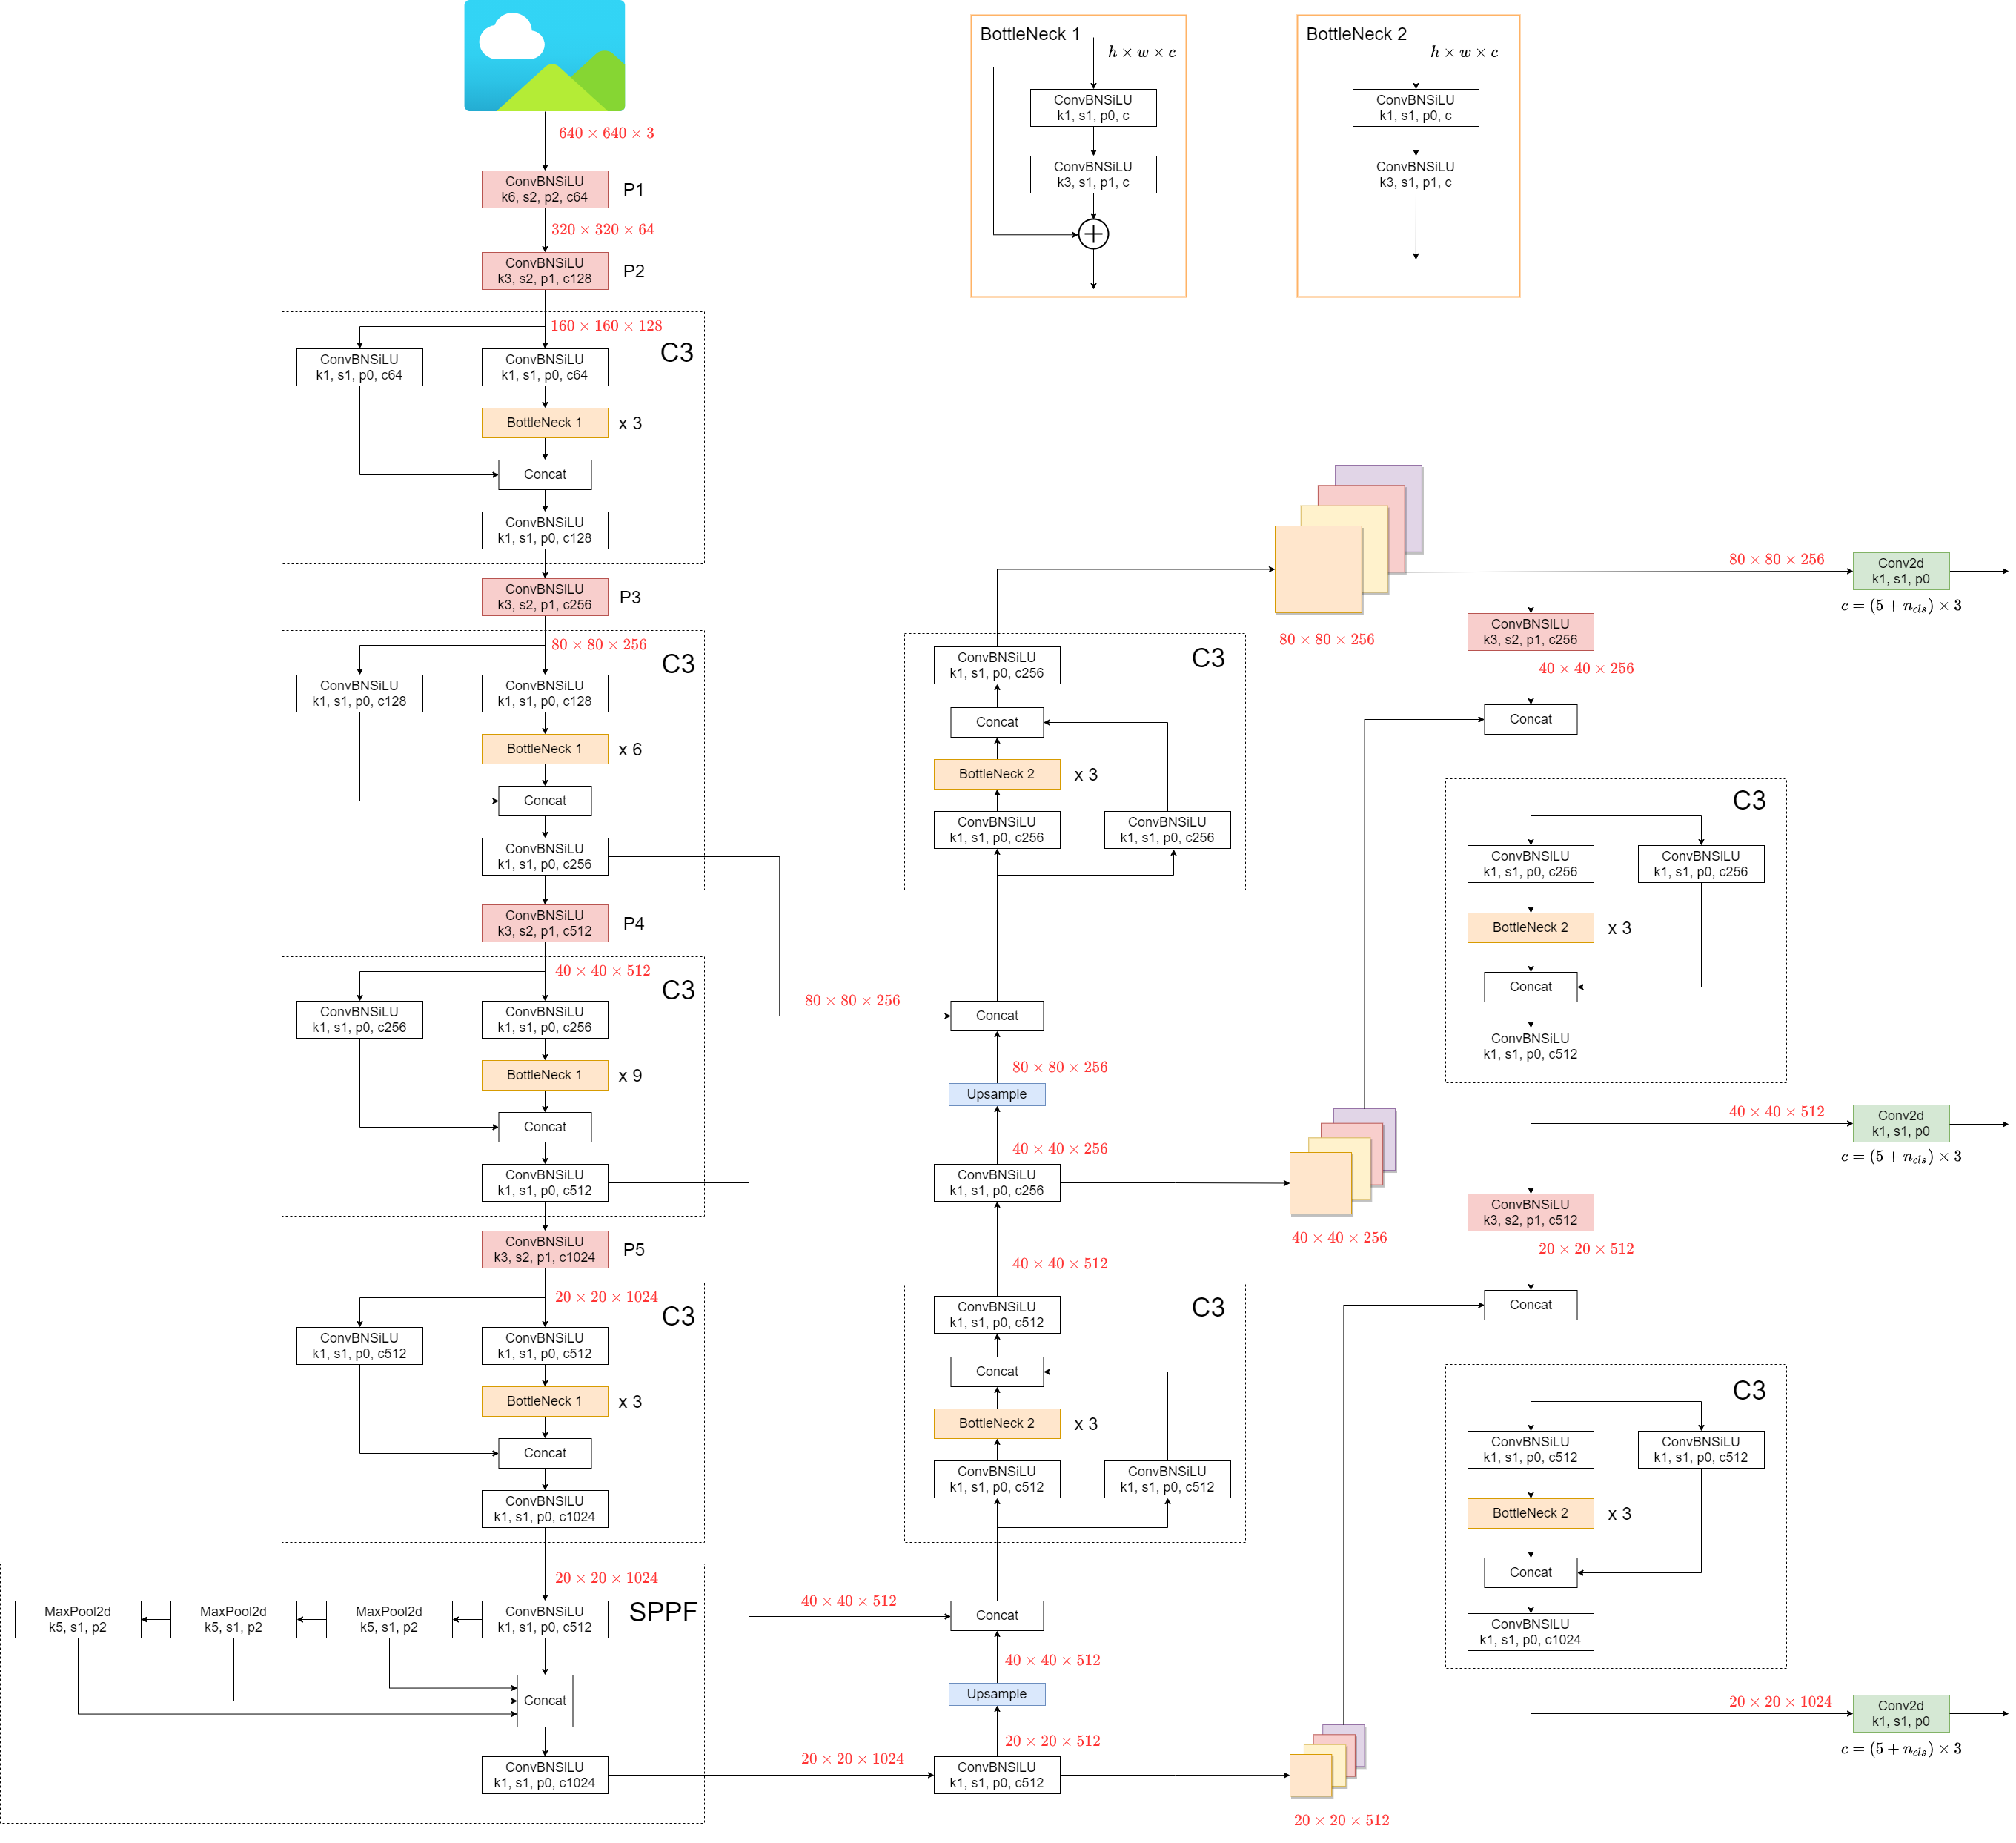
\includegraphics[width=1.0\linewidth]{images/a01-arch-yolov5}
	\caption[Architecture of YOLOv5.]{Architecture of YOLOv5~\cite{archYolov5}.}
	\label{fig:aa:archyolov5}
\end{figure}

\section{Instructions for validation and testing}

\begin{minipage}{\linewidth}
	\begin{lstlisting}[language=Bash, keywordstyle=\color{black}, 
		caption=General command to run the validation task of YOLOv5., label=lst:aa:valcmd]
		python val.py
			
			--weights <PATH_TO_PROJECT>/train/weights/best.pt
			
			--data <PATH_TO_DATASET>
			--project <PATH_TO_PROJECT>
			--name validation
			
			--batch-size 64
			--task val
			
			--save-txt
			--save-conf
			
			--device cuda:0
	\end{lstlisting}
\end{minipage}

\begin{minipage}{\linewidth}
	\begin{lstlisting}[language=Bash, keywordstyle=\color{black}, 
		caption=General command to run the testing task of YOLOv5., label=lst:aa:testcmd]
		python val.py
			
			--weights <PATH_TO_PROJECT>/train/weights/best.pt
			
			--data <PATH_TO_DATASET>
			--project <PATH_TO_PROJECT>
			--name test
			
			--batch-size 64
			--task test
			
			--save-txt
			--save-conf
			
			--device cuda:0
	\end{lstlisting}
\end{minipage}
